% Member 1 (T1). Figure: python -m project4.experiments.t1_expected_loss
\section{Decision theory with a reject option}
\label{sec:decision}

In section, we fix the loss matrix, find the action with the smallest expected loss,
and turn it into probability thresholds for our spam filter. Throughout,
$\post = \post(x) = \Prob(y=1\mid x)$ is the posterior probability that email $x$ is spam.

\subsection{Loss matrix}
\label{sec:loss-matrix}

The filter takes one of three actions: deliver ($a=0$), send to the spam folder ($a=1$), or hold for
human inspection ($a=r$). Table~\ref{tab:loss} gives the loss $L(a,y)$ of each action for each true label.

\begin{table}[ht]
\centering
\begin{tabular}{lcc}
\toprule
Action $\backslash$ true label & $y=0$ (real email) & $y=1$ (spam) \\
\midrule
$a=0$ deliver        & $0$     & $\cfn$ \\
$a=1$ spam folder    & $\cfp$  & $0$ \\
$a=r$ inspect        & $\ci$   & $\ci$ \\
\bottomrule
\end{tabular}
\caption{Loss matrix $L(a,y)$. Default values: $\cfp=10$, $\cfn=1$, $\ci=0.3$; the experiments sweep $\cfp/\cfn$ and $\ci$.}
\label{tab:loss}
\end{table}

\paragraph{Why these numbers.}
\begin{itemize}[itemsep=1pt,topsep=2pt]
  \item \emph{Correct decisions cost $0$.} Only relative losses matter, so we measure every loss against
        the outcome of a perfect filter.
  \item \emph{$\cfp=10$.} A real email in the spam folder is usually never seen: the reader may miss a
        reply, an invoice or a job offer. This is the worst outcome.
  \item \emph{$\cfn=1$.} A spam in the inbox costs a few seconds to recognise and delete. We use it as
        the unit of loss.
  \item \emph{$\ci=0.3$.} Held emails go to a review queue that a person scans in batches. Checking one
        is cheaper than dealing with a spam in the inbox, but not free. We take $0.3$ as a
        representative price: it lies well below the cut-off $\cstar$ of Section~\ref{sec:bayes-action},
        so inspection is worth using. The conclusions do not rest on this value, because
        Section~\ref{sec:accuracy-cost} treats every $\ci$.
\end{itemize}
Only the ratios $\cfp:\cfn:\ci$ affect the decisions, because multiplying every loss by a constant
does not change which action is cheapest.

\subsection{The cost-minimising action}
\label{sec:bayes-action}

For any loss matrix, the expected loss of action $a$ for an email with posterior $\post$ is
$R(a\mid x) = (1-\post)\,L(a,0) + \post\,L(a,1)$. Taking the action with the smallest $R(a\mid x)$
for every email also gives the smallest average loss over all emails; this is the Bayes action.
With Table~\ref{tab:loss},
\begin{equation}
  R(0\mid x) = \cfn\,\post, \qquad R(1\mid x) = \cfp\,(1-\post), \qquad R(r\mid x) = \ci .
  \label{eq:three-risks}
\end{equation}
Each is a straight line in $\post$, so the Bayes action depends on the email only through $\post$
and takes the form of thresholds on $\post$ (Figure~\ref{fig:t1-loss}).

\paragraph{Without inspection.}
The delivery line rises with $\post$ and the spam-folder line falls. They cross at
\[
  \tstar = \frac{\cfp}{\cfp+\cfn}, \qquad\text{where both equal}\qquad \cstar = \frac{\cfp\,\cfn}{\cfp+\cfn},
\]
so the filter delivers below $\tstar$ and sends to spam above it. The crossing is the worst case: an
email with $\post=\tstar$ has expected loss $\cstar$ whichever way the filter guesses, and no email
has a higher one.

\paragraph{With inspection.}
Near $\tstar$ the filter is effectively guessing, and either guess is expensive. Inspection replaces
the guess with a fixed price $\ci$ and the correct answer, so its line is flat and cuts off the peak
where the other two cross. This helps only if $0\le\ci<\cstar$; if $\ci\ge\cstar$ the flat line never
drops below both others, and the rule stays the single threshold $\tstar$. For $\ci<\cstar$ the inspect
line meets the delivery line at $\thz=\ci/\cfn$ and the spam-folder line at $\tho=1-\ci/\cfp$, so
\begin{equation}
  \text{deliver if } \post \le \thz = \frac{\ci}{\cfn}, \qquad
  \text{inspect if } \thz < \post < \tho, \qquad
  \text{spam folder if } \post \ge \tho = 1-\frac{\ci}{\cfp} .
  \label{eq:thresholds}
\end{equation}
At $\post=\thz$ and $\post=\tho$ two actions cost the same; the code breaks these ties towards the
automatic action.

\paragraph{Our costs.}
With $\cfp=10$ and $\cfn=1$, $\tstar=\cstar=10/11\approx0.909$. With $\ci=0.3$ the band exists and
$\thz = 0.3$, $\tho = 0.97$. The rule is strongly asymmetric: an email goes to the spam folder only if
the model is at least $97\%$ sure it is spam, because a wrong spam-folder decision costs ten times as
much as a wrong delivery. The lower threshold depends only on $\cfn$ and the upper one only on $\cfp$.

\paragraph{Sanity check: equal costs.}
With $\cfp=\cfn=c$ we get $\tstar=1/2$, $\cstar=c/2$, $\thz=\ci/c$ and $\tho=1-\ci/c$, so the filter
inspects iff $\max\{\post,1-\post\}<1-\ci/c$: when even the more likely label is not likely
enough. This is Chow's reject rule~\cite{chow1970,bishop2006}, and without inspection it is the
accuracy rule with threshold $1/2$. That rule is optimal only when $\cfp=\cfn$; with our costs the
threshold is $10/11$.

\begin{figure}[ht]
\centering
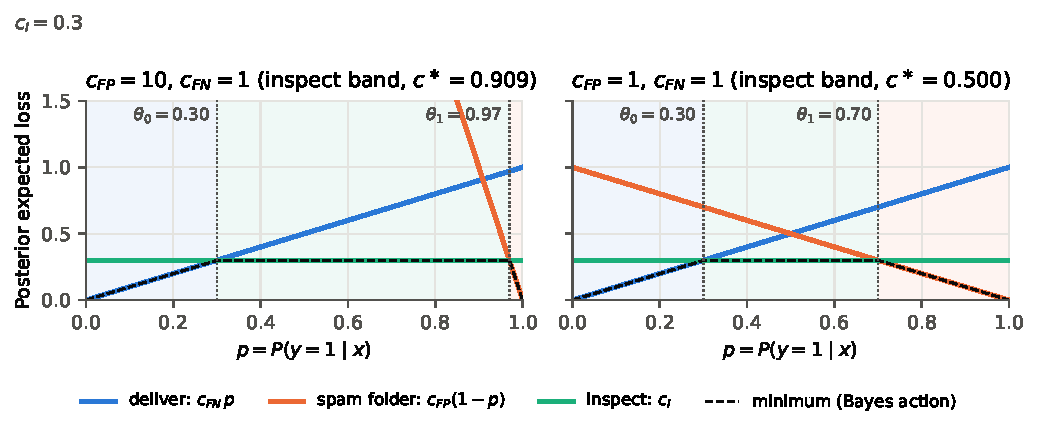
\includegraphics[width=\linewidth]{../project4/figures/t1_expected_loss.pdf}
\caption{Expected loss of each action against $\post$, with $\ci=0.3$. Shading shows where each action
is optimal. Left: our costs $\cfp=10$, $\cfn=1$, inspect band $(0.3,\,0.97)$. Right: equal costs
$\cfp=\cfn=1$, band $(0.3,\,0.7)$, symmetric about $\tstar=1/2$.
Generated by \texttt{experiments/t1\_expected\_loss.py}.}
\label{fig:t1-loss}
\end{figure}

\noindent These thresholds assume $\post$ is the true posterior; a model's estimate gives the Bayes
action only if it is calibrated (Section~\ref{sec:calibration}). The code implements
\eqref{eq:thresholds} in \texttt{decision.bayes\_action}, and a unit test checks it against a direct
minimisation over the three actions on $10{,}000$ random posteriors and loss matrices.

\subsection{The inspection assumption}
\label{sec:inspection}

So far inspection costs $\ci$ whatever the true label, and the inspector always finds the true label
and routes the email correctly. That is why the inspect row of Table~\ref{tab:loss} is constant and
its line in Figure~\ref{fig:t1-loss} is flat.

\paragraph{Variant: imperfect inspection.}
Suppose instead that the inspector sends a real email to spam with probability $\varepsilon_0$ and
delivers a spam with probability $\varepsilon_1$. The inspect row becomes
$L(r,0)=\ci+\varepsilon_0\cfp$ and $L(r,1)=\ci+\varepsilon_1\cfn$, so
$R(r\mid x)=\ci+\varepsilon_0\cfp(1-\post)+\varepsilon_1\cfn\,\post$ is a sloped line rather than a
flat one. It meets the delivery and spam-folder lines at
\[
  \thz' = \frac{\ci+\varepsilon_0\cfp}{(1-\varepsilon_1)\cfn+\varepsilon_0\cfp},
  \qquad
  \tho' = \frac{(1-\varepsilon_0)\cfp-\ci}{(1-\varepsilon_0)\cfp+\varepsilon_1\cfn}.
\]
For $\varepsilon_0=\varepsilon_1=0$ these are $\thz$ and $\tho$. Whenever the band exists
($\ci<\cfn$ is then automatic), $\thz'\ge\thz$ and $\tho'\le\tho$: an unreliable inspector is used for
fewer emails. We keep the perfect-inspection assumption in the rest of the report.
